\documentclass[twoside]{article}
\usepackage{graphicx}
\usepackage{amsmath}
\usepackage{listings}
\lstset{basicstyle=\ttfamily,escapeinside={||},columns=flexible}
\usepackage[colorlinks=true,allcolors=blue]{hyperref}
\usepackage{url}
\usepackage[top=.8in, bottom=.8in, left=0.9in, right=0.9in,a4paper]{geometry}

\begin{document}
\title{\textbf{MelodyShape: a Library and Tool for Symbolic Melodic Similarity based on Shape Similarity\\{\Large Version 1.4}}}
\author{Juli\'an Urbano\\Universitat Pompeu Fabra\\\texttt{urbano.julian@gmail.com}}
\maketitle

\sloppy 

\begin{abstract}
\noindent\texttt{MelodyShape}\footnote{For the latest version of the software and this document, please visit \url{https://github.com/julian-urbano/MelodyShape}.} is a Java library and tool to compute the melodic similarity between monophonic music pieces. It implements several algorithms that compute similarity based on the geometric shape that melodies describe in the pitch-time plane. All these algorithms have obtained the best results in the MIREX\footnote{\url{http://music-ir.org/mirex/wiki/MIREX_HOME}} Symbolic Melodic Similarity task in 2010, 2011, 2012, 2013, 2014 and 2015 editions, as well as the best results reported for the 2005 collection. This document describes the tool and its execution options; for background information the reader is referred to \cite{Urbano2011:shape}.
\end{abstract}

\section{Dependencies}

\texttt{MelodyShape} is available both as source code and as an executable JAR package. It requires two libraries found in the Apache Commons project, which are \emph{not} included in the JAR package: \texttt{commons-cli} and \texttt{commons-math}.
JAR packages for both libraries can be downloaded from the Apache Commons project website\footnote{\url{http://commons.apache.org}}. \texttt{MelodyShape} v1.4 was specifically implemented and tested with versions \texttt{commons-cli-1.3.1} and \texttt{commons-math3-3.6.1}.
Both libraries will have to be accessible from the Java classpath.

The easiest way to run the \texttt{MelodyShape} tool is to download all JAR files in the same directory, and then run Java from the command line (a graphical user interface is also available, see \S\ref{ssec:gui}.):
\begin{lstlisting}
$ ls
commons-cli-1.3.1.jar    commons-math3-3.6.1.jar    melodyshape-1.4.jar    data

$ java -jar melodyshape-1.4.jar
usage: melodyshape-1.4 -q <file/dir> -c <dir> -a <name> [-k <cutoff>] [-l]
                         [-t <num>] [-v] [-vv] [-gui] [-h]
-q <file/dir>  path to the query melody or melodies.
-c <dir>       path to the collection of documents.
-a <name>      algorithm to run:
               - 2010-domain, 2010-pitchderiv, 2010-shape
               - 2011-shape, 2011-pitch, 2011-time
               - 2012-shapeh, 2012-shapel, 2012-shapeg, 2012-time, 2012-shapetime
               - 2013-shapeh, 2013-time, 2013-shapetime
               - 2014-shapeh, 2014-time, 2014-shapetime
               - 2015-shapeh, 2015-time, 2015-shapetime
-k <cutoff>    number of documents to retrieve.
-l             show results in a single line (omits similarity scores).
-t <num>       run a fixed number of threads.
-v             verbose, to stderr.
-vv            verbose a lot, to stderr.
-gui           run with graphical user interface.
-h             show this help message.

MelodyShape 1.4  Copyright (C) 2013-2016  Julian Urbano <urbano.julian@gmail.com>
This program is distributed under the terms of the MIT License.
\end{lstlisting}

Alternatively, one can use Maven to build the project and, in particular, download dependencies directly.
\begin{lstlisting}
$ mvn dependency:copy-dependencies
...
$ ls target/dependencies
commons-cli-1.3.1.jar  commons-math3-3.6.1.jar
\end{lstlisting}

Currently, \texttt{MelodyShape} v1.4 is compiled for Java 7. It can be redistributed and/or modified under the terms of the MIT License.

\section{Tool Options}

\subsection{Basic Execution}

\texttt{MelodyShape} requires one or more query melodies, a collection of melodies to sort according to their melodic similarity to the queries, and the name of the algorithm to compute those similarities. These three parameters must be indicated with arguments \texttt{-q}, \texttt{-c} and \texttt{-a} in the command line. For instance, we can compute the similarity of melody \texttt{data/q01.mid} with all melodies in directory \texttt{data/coll/} using algorithm \texttt{2010-shape}:
\begin{lstlisting}
$ java -jar melodyshape-1.4.jar -q data/q01.mid -c data/coll/ -a 2010-shape
06C6.mid    0.48583945
1065.mid    0.16715906
07D0.mid    0.15722630
0A5A.mid    0.14412330
04D7.mid    0.10835528
...
\end{lstlisting}

The output is a list of all files in \texttt{data/coll/} sorted by melodic similarity to the query in descending order, along with the computed similarity score. Note that all files must have extension \texttt{.mid} or \texttt{.midi}. In addition, only one MIDI pitch can be on at any point in time.

\subsection{Several Queries}

\texttt{MelodyShape} can be run several times, once for each of the queries we have. Alternatively, it can be run once for all queries, resulting in a more efficient execution. The following would run \texttt{MelodyShape} will all queries in directory \texttt{data/}\footnote{Throughout this document, underlined text highlights the changes with the previous executions.}:
\begin{lstlisting}
$ java -jar melodyshape-1.4.jar |\underline{-q data/}| -c data/coll/ -a 2010-shape
q01.mid    06C6.mid    0.48583945
q01.mid    1065.mid    0.16715906
...
q01.mid    0C29.mid    -0.18696516
q02.mid    0859.mid    0.44796066
...
q06.mid    0B63.mid    -0.19795232
q06.mid    0EA2.mid    -0.22072806
\end{lstlisting}

Results are again sorted by melodic similarity to the queries, one query after another. The first column identifies the query file, the second column identifies the document and the third column shows the computed similarity score.

\subsection{Cutoff: \texttt{-k}}

The \texttt{-k} command line argument can be used to indicate how many results to show per query. For example, to show only the two most similar melodies for each query:
\begin{lstlisting}
$ java -jar melodyshape-1.4.jar -q data/ -c data/coll/ -a 2010-shape |\underline{-k 2}|
q01.mid    06C6.mid    0.48583945
q01.mid    1065.mid    0.16715906
q02.mid    0859.mid    0.44796066
q02.mid    03FA.mid    0.18388982
...
q06.mid    0859.mid    0.26747611
q06.mid    0B15.mid    0.24436125
\end{lstlisting}

\subsection{Single Line: \texttt{-l}}

The \texttt{-l} command line argument indicates that results should be displayed in a single line, one line per query:
\begin{lstlisting}
$ java -jar melodyshape-1.4.jar -q data/ -c data/coll/ -a 2010-shape |\underline{-k 5}| |\underline{-l}|
q01.mid    06C6.mid    1065.mid    07D0.mid    0A5A.mid    04D7.mid
q02.mid    0859.mid    03FA.mid    0B15.mid    0454.mid    0B2C.mid
...
q06.mid    0859.mid    0B15.mid    0F0A.mid    0B2C.mid    0454.mid
\end{lstlisting}

Similarly, the first column identifies the query, and the rest identifies the most similar melodies in the collection, from left to right.

\subsection{Verbose: \texttt{-v} and \texttt{-vv}}

The \texttt{-v} command line argument can be used to display the execution progress, simply showing when each query starts being run:
\begin{lstlisting}
$ java -jar melodyshape-1.4.jar -q data/ -c data/coll/ -a 2010-shape -k 5 -l |\underline{-v}|
(1/6) q01.mid...done.
q01.mid    06C6.mid    1065.mid    07D0.mid    0A5A.mid    04D7.mid
(2/6) q02.mid...done.
q02.mid    0859.mid    03FA.mid    0B15.mid    0454.mid    0B2C.mid
...
(6/6) q06.mid...done.
q06.mid    0859.mid    0B15.mid    0F0A.mid    0B2C.mid    0454.mid
\end{lstlisting}

The \texttt{-vv} command line argument can be used to display real-time execution progress, some information about the algorithm used and time spent running each query:
\begin{lstlisting}
$ java -jar melodyshape-1.4.jar -q data/ -c data/coll/ -a 2010-shape -k 5 -l |\underline{-vv}|
Reading queries...done (6 melodies).
Reading collection...done (2000 melodies).
Instantiating algorithm...done.
  Comparer: nGram(3,Hybrid(Cache(Freq(BSplineShape(8.0,1.0,0.5)))))
    Ranker: Untie(nGram(3,Hybrid(Eq)))
   Threads: 4
 
(1/6) q01.mid: [========================] 100% comparing...ranking...done (3 sec).
q01.mid    06C6.mid    1065.mid    07D0.mid    0A5A.mid    04D7.mid
(2/6) q02.mid: [========================] 100% comparing...ranking...done (2 sec).
q02.mid    0859.mid    03FA.mid    0B15.mid    0454.mid    0B2C.mid
...
(6/6) q06.mid: [============>                ]  51% comparing...
\end{lstlisting}

All this extra information is output to the standard error stream, so that the actual results per query can be easily set apart with a pipeline:
\begin{lstlisting}
$ java -jar melodyshape-1.4.jar -q data/ -c data/coll/ -a 2010-shape -l -vv |\underline{> out}|
Reading queries...done (6 melodies).
Reading collection...done (2000 melodies).
Instantiating algorithm...done.
  Comparer: nGram(3,Hybrid(Cache(Freq(BSplineShape(8.0,1.0,0.5)))))
    Ranker: Untie(nGram(3,Hybrid(Eq)))
   Threads: 4
 
(1/6) q01.mid: [========================] 100% comparing...ranking...done (3 sec).
(2/6) q02.mid: [========================] 100% comparing...ranking...done (2 sec).
...
(6/6) q06.mid: [========================] 100% comparing...ranking...done (4 sec).

$ cat out
q01.mid    06C6.mid    1065.mid    07D0.mid    0A5A.mid    04D7.mid ...
q02.mid    0859.mid    03FA.mid    0B15.mid    0454.mid    0B2C.mid ...
...
q06.mid    0859.mid    0B15.mid    0F0A.mid    0B2C.mid    0454.mid ...
\end{lstlisting}

\subsection{Number of Threads: \texttt{-t}}

The \texttt{-t} command line argument can be used to indicate the number of threads to use by the algorithms. By default, as many threads as CPU cores found in the machine will be used. We can, for instance, restrict CPU usage to just two threads:
\begin{lstlisting}
$ java -jar melodyshape-1.4.jar -q data/ -c data/coll/ -a 2010-shape |\underline{-t 2}|
\end{lstlisting}

\subsection{Graphical User Interface: \texttt{-gui}}\label{ssec:gui}

The \texttt{-gui} command line argument can be used to run \texttt{MelodyShape} with a graphical user interface rather than as a command line tool, which will show up a window as in Figure~\ref{fig:gui}. Alternatively, the graphical user interface can be run directly by running the \texttt{melodyshape-1.4.jar} JAR file from a windows or file explorer, usually by double-clicking on it.
\begin{figure}[!h]
\centering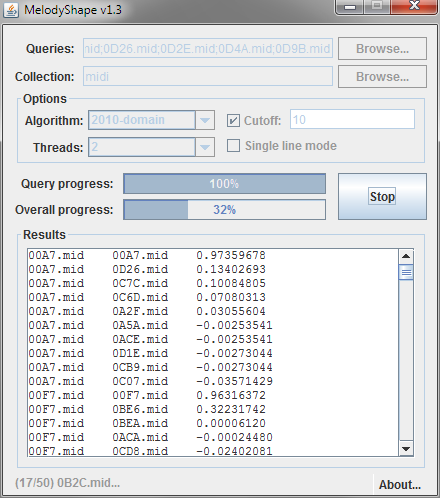
\includegraphics[scale=.6]{gui.png}
\caption{\texttt{MelodyShape} graphical user interface.}
\label{fig:gui}
\end{figure}

The options available from the graphical user interface are basically those available from the command line. The user can copy the results to the system clipboard by right-clicking on the results panel and selecting the \texttt{Copy All} option.

\section{Algorithms}

\texttt{MelodyShape} implements several melodic similarity algorithms based on a geometric model that represents melodies as spline curves in the pitch-time plane. The similarity between two melodies is then computed with a sequence alignment algorithm between sequences of spline spans: the more similar the shape of the curves, the more similar the melodies they represent. \texttt{MelodyShape} v1.4 implements algorithms based on this model that have been submitted to the MIREX Symbolic Melodic Similarity task in 2010, 2011, 2012, 2013, 2014 and 2015. 

The following table shows the \texttt{-a} command line argument to be used for each algorithm, with the corresponding official MIREX submission name\footnote{Algorithm \textsf{JU3-ParamDeriv} from MIREX 2010 is not implemented in \texttt{MelodyShape}.}. For instance, argument \texttt{-a 2011-shape} corresponds to algorithm \textsf{UL1-Shape} from MIREX 2011, which is the same as algorithms \textsf{JU4-Shape}, \textsf{ULMS1-ShapeH}, \textsf{JU1-ShapeH}, \textsf{JU1-ShapeH} and \textsf{JU1-ShapeH} from MIREX 2010, 2012, 2013, 2014 and 2015, respectively.

\begin{table}[!h]\setlength{\tabcolsep}{4pt}
\small\centering\begin{tabular}{l|llll}
	\hline
	\texttt{-a} argument     & MIREX 2010              & MIREX 2011         & MIREX 2012               & MIREX 2013--2015             \\ \hline
	\texttt{2010-domain}     & \textsf{JU1-Domain}     &                    &                          &                        \\
	\texttt{2010-pitchderiv} & \textsf{JU2-PitchDeriv} &                    &                          &                        \\
	\texttt{2010-shape}      & \textsf{JU4-Shape}      & \textsf{UL1-Shape} & \textsf{ULMS1-ShapeH}    & \textsf{JU1-ShapeH}    \\ \hline
	\texttt{2011-shape}      & \textsf{JU4-Shape}      & \textsf{UL1-Shape} & \textsf{ULMS1-ShapeH}    & \textsf{JU1-ShapeH}    \\
	\texttt{2011-pitch}      &                         & \textsf{UL2-Pitch} &                          &                        \\
	\texttt{2011-time}       &                         & \textsf{UL3-Time}  & \textsf{ULMS5-Time}      & \textsf{JU3-Time}      \\ \hline
	\texttt{2012-shapeh}     & \textsf{JU4-Shape}      & \textsf{UL1-Shape} & \textsf{ULMS1-ShapeH}    & \textsf{JU1-ShapeH}    \\
	\texttt{2012-shapel}     &                         &                    & \textsf{ULMS2-ShapeL}    &                        \\
	\texttt{2012-shapeg}     &                         &                    & \textsf{ULMS3-ShapeG}    &                        \\
	\texttt{2012-time}       &                         & \textsf{UL3-Time}  & \textsf{ULMS5-Time}      & \textsf{JU3-Time}      \\
	\texttt{2012-shapetime}  &                         &                    & \textsf{ULMS4-ShapeTime} & \textsf{JU2-ShapeTime} \\ \hline
	\texttt{2013-shapeh}     & \textsf{JU4-Shape}      & \textsf{UL1-Shape} & \textsf{ULMS1-ShapeH}    & \textsf{JU1-ShapeH}    \\
	\texttt{2013-time}       &                         & \textsf{UL3-Time}  & \textsf{ULMS5-Time}      & \textsf{JU3-Time}      \\
	\texttt{2013-shapetime}  &                         &                    & \textsf{ULMS4-ShapeTime} & \textsf{JU2-ShapeTime} \\ \hline
	\texttt{2014-shapeh}     & \textsf{JU4-Shape}      & \textsf{UL1-Shape} & \textsf{ULMS1-ShapeH}    & \textsf{JU1-ShapeH}    \\
	\texttt{2014-time}       &                         & \textsf{UL3-Time}  & \textsf{ULMS5-Time}      & \textsf{JU3-Time}      \\
	\texttt{2014-shapetime}  &                         &                    & \textsf{ULMS4-ShapeTime} & \textsf{JU2-ShapeTime} \\ \hline
	\texttt{2015-shapeh}     & \textsf{JU4-Shape}      & \textsf{UL1-Shape} & \textsf{ULMS1-ShapeH}    & \textsf{JU1-ShapeH}    \\
	\texttt{2015-time}       &                         & \textsf{UL3-Time}  & \textsf{ULMS5-Time}      & \textsf{JU3-Time}      \\
	\texttt{2015-shapetime}  &                         &                    & \textsf{ULMS4-ShapeTime} & \textsf{JU2-ShapeTime} \\ \hline
\end{tabular}
\end{table}

The reader is referred to the corresponding MIREX participation report for a detailed description of each of these algorithms \cite{Urbano2010:mirex2010,Urbano2011:mirex2011,Urbano2012:mirex2012,Urbano2013:mirex2013,Urbano2014:mirex2014,Urbano2015:mirex2015}. For a general description of the geometric model, please refer to \cite{Urbano2011:shape}.

\section*{Acknowledgments}
This work is supported by an A4U postdoctoral grant and a Juan de la Cierva postdoctoral fellowship.

\bibliographystyle{plain}
\bibliography{melodyshape}

\end{document}
